\documentclass[a4paper,12pt,draft]{article}

\usepackage[utf8]{inputenc}
\usepackage[T1]{fontenc}
\usepackage{amssymb}
\usepackage{amsmath}
\usepackage{epigraph}						% Funny quotes
\usepackage{bm}								% Bold face for vectors/matrices
\usepackage[hidelinks]{hyperref}			% Invisible, clickable links in pdf
\usepackage{listings}						% Display source code nicely
\usepackage{mcode}							% Ditto MATLAB code
\usepackage{algpseudocode}					% Nice Al Gore Rhythms
\usepackage{graphicx}						% Including graphics
\usepackage{epstopdf}						% Self-explanatory
\usepackage{float} 							% Better float placing (H option)
\usepackage{siunitx}						% SI units
\bibliographystyle{ieeetr}					% Citations in IEEE style
\lstset{frame=topbottom}

\newcommand{\M}[1]{\bm{#1}} 				% Use for variable matrices
\newcommand{\Mc}[1]{\mathbf{#1}} 			% Use for constant matrices (I, etc.)
\newcommand{\V}[1]{\mathbf{#1}} 			% Use for vectors
\newcommand{\transpose}{^{\text{T}}} 		% Make a guess, bitch
\newcommand{\sub}[1]{_{\textnormal{#1}}} 	% For upright subscripts

\lstset{
    frame=single,
    breaklines=true,
    postbreak=\raisebox{0ex}[0ex][0ex]{\ensuremath{\color{green}\hookrightarrow\space}},
    morekeywords={model, import, constant, parameter, equation, end},
    keywordstyle=\color{blue},
    numbers=left,
    numberstyle=\scriptsize,
    stepnumber=1,
    numbersep=8pt
}

\begin{document}

\begin{titlepage}
\begin{center}

\textsc{\LARGE TTK4135}\\[1.5cm]
\textsc{\LARGE Report} \linebreak
{ \huge \bfseries \textcolor[rgb]{0,0,1}{Helicopter Lab}\\[0.5cm] }
\today \vspace{1cm} \linebreak 
\emph{\textbf{Student numbers:}} \linebreak 
742434 \linebreak
XXXXXX \linebreak
XXXXXX \linebreak
XXXXXX \linebreak
XXXXXX \linebreak\linebreak \textbf{Group 9}  \vspace{3cm}\linebreak \linebreak

\textsc{Faculty of Information Technology, Mathematics and Electrical Engineering}\linebreak
\textsc{Department of Engineering Cybernetics} 
\vfill


\includegraphics[width=200pt, keepaspectratio=true]{logo_ntnu_eng.eps}

\end{center}
\end{titlepage}
\begin{abstract}

This is a report for the mandatory lab exercise in the course TTK4135 Optimization and Control held at NTNU the spring 2015. The purpose of this exercise is to get practical experience in formulating dynamic optimization problems, discretizise them and solve them using a computer, as well as using these results to impliment optimal controllers with and without feedback. The optimization problems that got solved were quadratic minimization problems, and the feedback was introduced using LQ controllers.

\end{abstract}

\tableofcontents

\section{Introduction}

The intention of this lab assignment is to apply various optimisation-based control techniques to a physical model of a helicopter. The system with its hardware is described in detail in \cite{_helicopter_2015}. A mathematical model of the helicopter with pitch and elevation controllers is already made for us. Our objective is to find an optimal sequence of inputs that will steer the helicopter on the desired path. This will be done by formulating optimization problems, and solving them. We will solve them as discrete problems using MATLAB, which mean that we first have to discretise our system. We apply this input sequence to the system using Simulink/QuaRC. We then run the helicopter using the optimal input directly, and compare the behaviour to when we introduce feedback.

In this report we will be presenting our results in the same order that they were obtained, meaning we will have one section for each exercise in \cite{_helicopter_2015}, where the relevant mathematics, code, plots, results, and so on will be added. The discussion will be done alongside this, with the exception of one summarizing discussion at the end of the report. 
\section{Repetition/introduction to Simulink/QuaRC (10.1)}

The first exercise in the exercise set was meant as a repetition for those that have completed the Helicopter lab in the course TTK4115 Linear System Theory, and a introduction to Simulink/QuaRC for the rest. In our group everyone have completed the lab from TTK4115, and we didn't use much time on this problem. We ran the Simulink/QuaRC-program, and observed that premade controllers were behaving fine. We changed the setpoints in real-time, and immediately got satisfying responses from the helicopter.
\epigraph{\textit{'Smack my pitch up.'}}{The Prodigy (1997)}

\section{Optimal control of pitch/travel without feedback (10.2)}

%%%%%%%%%%%%%%%%%%%%%%%%%%%%%%%%%%%%%%%%%%%%%%%%%%%%%%%%%%%%
\subsection{State space form (10.2.1)}
%%%%%%%%%%%%%%%%%%%%%%%%%%%%%%%%%%%%%%%%%%%%%%%%%%%%%%%%%%%%
We want to write the model \eqref{eq:model1} in continuous time state space form with states and input as shown in \eqref{eq:state_and_input} below.

\begin{equation}\label{eq:model1}
	\V{\dot{x}} = \M{A}_{c}\V{x} + \M{B}_{c}u
\end{equation}

\begin{equation}\label{eq:state_and_input}
\begin{aligned}
	\V{x} 	&= \begin{bmatrix}\lambda & r & p & \dot{p} \end{bmatrix}\transpose \\
	u 		&= p_{c}
\end{aligned}
\end{equation}
The equations of motion for the states are shown in \eqref{eq:state_equations} and the constants used are defined in \eqref{eq:K1K2}. (These are derived in detail in \cite{_helicopter_2015}, and will not be further explained here. The same applies for \eqref{eq:state_eqns} in section \ref{10.4.1}.)

\begin{equation}\label{eq:state_equations}
\begin{aligned}
	\dot{\lambda} 	&= r \\
	\dot{r} 		&= - K_{a} p \\
	\dot{p} 		&= \dot{p} \\
	\ddot{p} 		&= K_{1} K_{pp} (p_{c} - p) - K_{1} K_{pd} \dot{p}
\end{aligned}
\end{equation}

\begin{equation}\label{eq:K1K2}
\begin{aligned}
	K_{1} &= \frac{K_{f} l_{n}}{J_{p}} \\
	K_{2} &= \frac{K_{p} l_{a}}{J_{t}}
\end{aligned}
\end{equation}
The above gives the result in \eqref{eq:state_space_matrices}.

\begin{equation}\label{eq:state_space_matrices}
	\V{\dot{x}} =
	\underbrace{
		\begin{bmatrix}
			0 & 1 & 0 				& 0 \\
			0 & 0 & -K_{2} 			& 0 \\
			0 & 0 & 0 				& 1 \\
			0 & 0 & -K_{1}K_{pp}	& -K_{1}K_{pd}
		\end{bmatrix}
	}_{\M{A}_{c}}
	\V{x} +
	\underbrace{
		\begin{bmatrix}
			0 \\ 0 \\ 0 \\ K_{1}K_{pp}
		\end{bmatrix}
	}_{\M{B}_{c}}
	u
\end{equation}


%%%%%%%%%%%%%%%%%%%%%%%%%%%%%%%%%%%%%%%%%%%%%%%%%%%%%%%%%%%%
\subsection{Model discussion (10.2.1)}
%%%%%%%%%%%%%%%%%%%%%%%%%%%%%%%%%%%%%%%%%%%%%%%%%%%%%%%%%%%%
The system states are travel, travel rate, pitch, and pitch rate. The output of our controller is the pitch setpoint to be used by the already implemented controller, which in turn calculates voltage inputs for the hardware. We are therefore not modelling the helicopter alone, but a larger system consistinf of the helicopter along with the given controller. This corresponds with figure 7 in the exercise text \cite{_helicopter_2015}.


%%%%%%%%%%%%%%%%%%%%%%%%%%%%%%%%%%%%%%%%%%%%%%%%%%%%%%%%%%%%
\subsection{Discretisation (10.2.2)}\label{sec:disc1}
%%%%%%%%%%%%%%%%%%%%%%%%%%%%%%%%%%%%%%%%%%%%%%%%%%%%%%%%%%%%
We discretise the system by the Forward Euler Method. The general definition of the method and how it relates to our system is described by equations \eqref{eq:forward_euler} and \eqref{eq:euler_func}, respectively.

\begin{equation}\label{eq:forward_euler}
	y_{k+1} = y_{k} + h f(x_{k}, y_{k})
\end{equation}

\begin{equation}\label{eq:euler_func}
	f = \left( \M{A}_{c} \V{x}_{k} + \M{B}_c u_{k} \right)
\end{equation}
Using \eqref{eq:forward_euler} and \eqref{eq:euler_func}, we can determine the matrices of the discrete system, as shown in \eqref{eq:disc}, \eqref{eq:disc_matrix_A}, and \eqref{eq:disc_matrix_B}.

\begin{equation}\label{eq:disc}
\begin{aligned}
	\V{x}_{k+1} &= \V{x}_{k} + \left( \M{A}_{c} \V{x}_{k} + \M{B}_c u_{k} \right) h \\
				&= \V{x}_{k} + h\M{A}_{c}\V{x}_{k} + h\M{B}_{c}u_{k} \\
				&= \left( \Mc{I} + h\M{A}_{c} \right) \V{x}_{k} + h\M{B}_{c}u_{k} \\
				&= \M{A}\V{x}_{k} + \M{B}u_{k}
\end{aligned}
\end{equation}

\begin{equation}\label{eq:disc_matrix_A}
	\M{A} = \Mc{I} + h\M{A}_{c} =
	\begin{bmatrix}
		1 & h & 0 & 0 \\
		0 & 1 & -K_{2}h & 0 \\
		0 & 0 & 1 & h \\
		0 & 0 & -K_{1}K_{pp}h	& 1-K_{1}K_{pd}h
	\end{bmatrix}
\end{equation}

\begin{equation}\label{eq:disc_matrix_B}
	\M{B} = h\M{B}_c =
	\begin{bmatrix} 0 \\ 0 \\ 0 \\ K_{1}K_{pp}h \end{bmatrix}
\end{equation}


%%%%%%%%%%%%%%%%%%%%%%%%%%%%%%%%%%%%%%%%%%%%%%%%%%%%%%%%%%%%
\subsection{Discussion of the cost function (10.2.3)}
%%%%%%%%%%%%%%%%%%%%%%%%%%%%%%%%%%%%%%%%%%%%%%%%%%%%%%%%%%%%
The assignment text specifies a cost function \eqref{eq:cost_function} \cite{_helicopter_2015} that we want to minimise subject to the constraints given in \eqref{eq:cost_constraint}.


\begin{equation} \label {eq:cost_function}
	\phi = \sum\limits_{i=1}^N (\lambda_i - \lambda_f)^2 + q p_{ci}^2, \quad q \geq 0 
\end{equation}

\begin{equation} \label{eq:cost_constraint}
	|p_k| \leq \frac{30 \pi}{180}, \quad k \in \{ 1, ..., N \}
\end{equation}

This cost function focuses on the error between $\lambda_i$ and $\lambda_f$.
It is a least-square (i.e. quadratic) function and can therefore be solved by quadratic programming methods.
The second term of the cost function involves the pitch setpoint, which is weighed by a constant $q$.


%%%%%%%%%%%%%%%%%%%%%%%%%%%%%%%%%%%%%%%%%%%%%%%%%%%%%%%%%%%%
\subsection{Procedure for solving the optimization problem (10.2.3)}
\label{optimalProcedure}
%%%%%%%%%%%%%%%%%%%%%%%%%%%%%%%%%%%%%%%%%%%%%%%%%%%%%%%%%%%%

The intention is to calculate an optimal helicopter trajectory between $x_0 = \begin{bmatrix} \lambda_0 & 0 & 0 & 0 \end{bmatrix} \transpose$ and $x_f = \begin{bmatrix} \lambda_f & 0 & 0 & 0 \end{bmatrix} \transpose$, while assuming a constant elevation angle. In this case we use $\lambda_0 = \pi$ and $\lambda_f = 0$.

We first declare the constants given in Table \ref{table:constants}, the $\M{A}$ and $\M{B}$ matrices given in \eqref{eq:state_space_matrices}, and $x_0$ given above. Then we implement the constraints in \eqref{eq:cost_constraint} using the following code:

\begin{lstlisting}
% Bounds

ul 	    = -30*pi/180;        % Lower bound on control -- u1
uu 	    = 30*pi/180;         % Upper bound on control -- u1

xl      = -Inf*ones(mx,1);   % Lower bound on states (no bound)
xu      = Inf*ones(mx,1);    % Upper bound on states (no bound)
xl(3)   = ul;                % Lower bound on state x3
xu(3)   = uu;                % Upper bound on state x3

% Generate constraints on measurements and inputs

[vlb,vub]       = genBegr2(N,M,xl,xu,ul,uu);
vlb(N*mx+M*mu)  = 0;         % We want the last input to be zero
vub(N*mx+M*mu)  = 0;         % We want the last input to be zero

\end{lstlisting}
where \texttt{genBegr2} is like this:

%NB denne koden er hentet fra nettet, skriv kilde
\vspace{1cm}
\begin{lstlisting} %få kommentarene på en linje, ser mye bedre ut

function [vlb,vub] = genBegr2(N,M,xl,xu,ul,uu);

vlb_x	= repmat(xl,N,1);	% Lager begrensning for hvert tidsskritt
vub_x	= repmat(xu,N,1);	% Lager begrensning for hvert tidsskritt

vlb_u	= repmat(ul,M,1);	% Lager begrensning for hvert tidsskritt
vub_u	= repmat(uu,M,1);	% Lager begrensning for hvert tidsskritt

vlb	    = [vlb_x; vlb_u];	% Setter sammen begrensningene for xl og ul
vub	    = [vub_x; vub_u];	% Setter sammen begrensningene for xu og uu
\end{lstlisting}

After that we find weight matrices for the QP problem and the matrices for the equality constrains:
\begin{lstlisting}
% Generate the matrix Q and the vector c (objecitve function weights in the QP problem) 

Q1 = zeros(mx,mx);
Q1(1,1) = 1;                	% Weight on state x1
Q1(2,2) = 0;                	% Weight on state x2
Q1(3,3) = 0;                	% Weight on state x3
Q1(4,4) = 0;                	% Weight on state x4
P1 = q;                     	% Weight on input
Q = 2*genq2(Q1,P1,N,M,mu);  	% Generate Q
c = zeros(N*mx+M*mu,1);     	% Generate c

% Generate system matrixes for linear model

Aeq = gena2(A1,B1,N,mx,mu); 	% Generate A
beq = zeros(1, size(Aeq,1));	% Generate b
beq(1:mx) = A1*x0; 	        	% Initial value
\end{lstlisting}
using \texttt{genq2} 

\begin{lstlisting} %NB denne koden er hentet fra nettet, skriv kilde

function Q = genq2(Q1,P1,N,M,mu)

p1	= blkdiag2(P1,M);
q1	= blkdiag2(Q1,N);

Q	= blkdiag(q1,p1); 
\end{lstlisting}
and \texttt{gena2}

\begin{lstlisting} %NB denne koden er hentet fra nettet, skriv kilde

function A = gena2(A1,B1,N,mx,mu)

A 	= zeros(N*mx,N*mx+N*mu);
b1	= blkdiag2(-B1,N);
a1	= eye(N*mx);
for i=1:(N-1)
  a1([(i*mx+1):((i+1)*mx)],[((i-1)*mx+1):(i*mx)])=-A1;
end
A	= [a1 b1];
\end{lstlisting}

At last we solve the quadratic problem using the MATLAB command \texttt{quadprog}:

\begin{lstlisting}
	[z,lambda] = quadprog(Q, c, [], [], Aeq, beq, vlb, vub, z0);
\end{lstlisting}
where $\M{Z} = \begin{bmatrix} \V{x}_1 & \V{x}_2 & ... & \V{x}_N & u_1 & u_2 & ... & u_N \end{bmatrix} \transpose$. The full code is listed in the appendix. We extract the desired states and get the following plots, using three different values of $q$:


\begin{figure}[H]
        \centering
        \begin{subfigure}[b]{0.5\textwidth}
                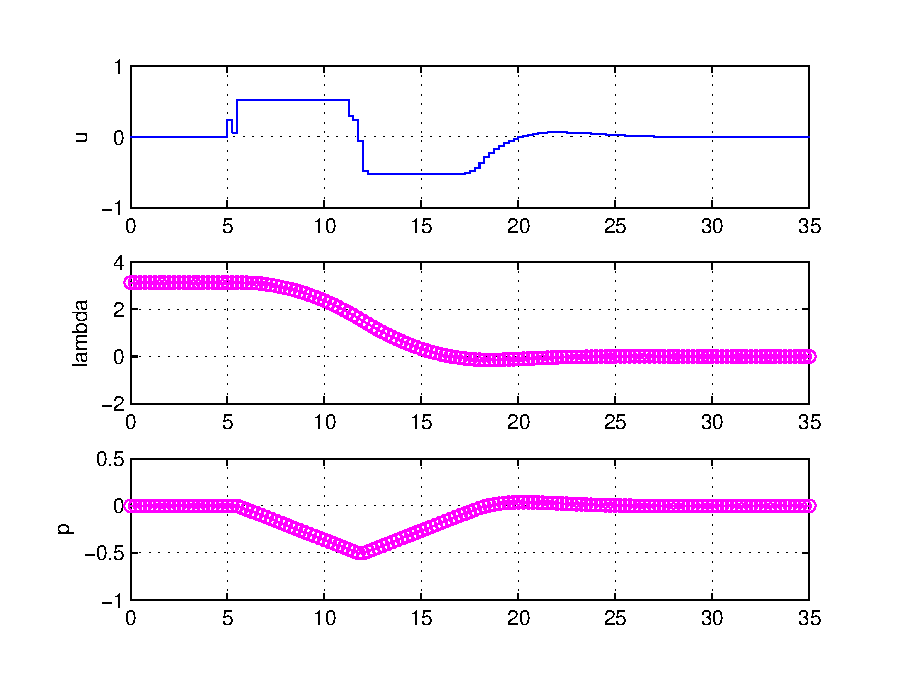
\includegraphics[width=\textwidth]{day2q0komma1}
                \caption{Optimal path with $q = 0.1$}
                \label{fig:estimatedDay201}
        \end{subfigure}%
        ~ 
        \begin{subfigure}[b]{0.5\textwidth}
                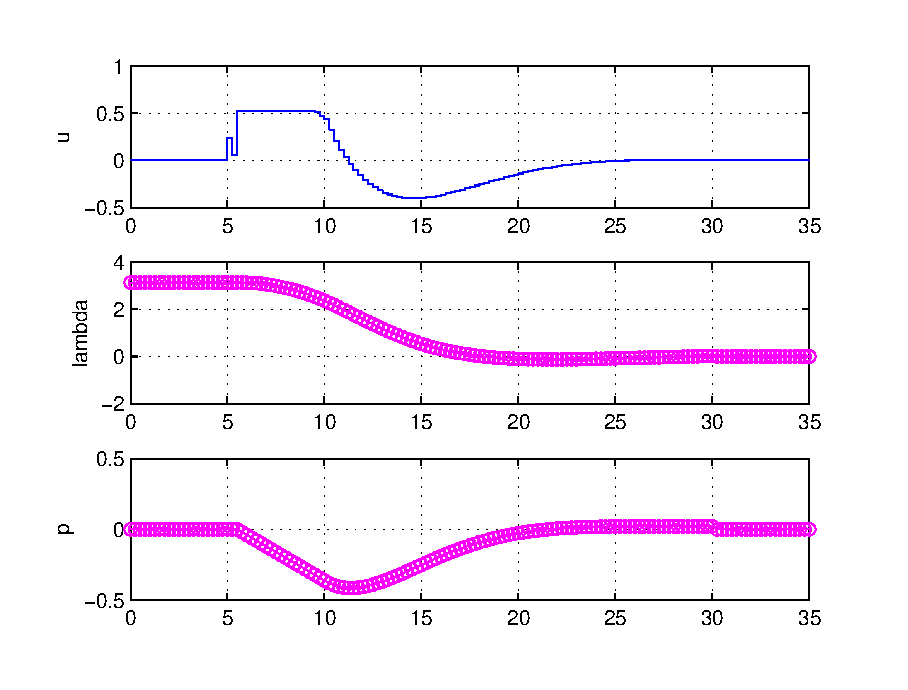
\includegraphics[width=\textwidth]{day2q1}
                \caption{Optimal path with $q = 1$}
                \label{fig:estimatedDay202}
        \end{subfigure}
        ~ 
        \begin{subfigure}[b]{0.5\textwidth}
                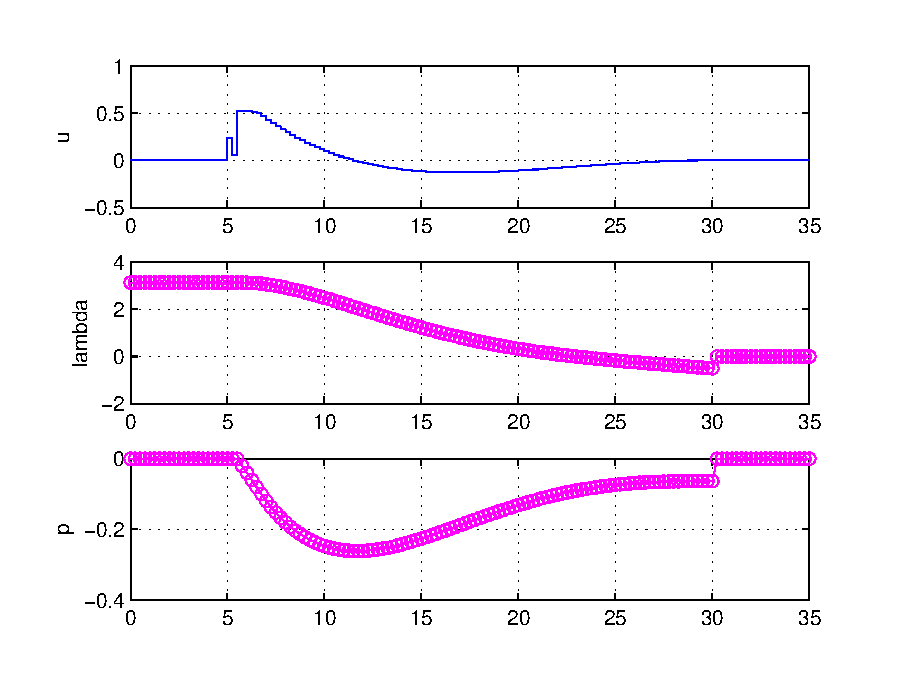
\includegraphics[width=\textwidth]{day2q10}
                \caption{Optimal path with $q = 10$}
                \label{fig:estimatedDay203}
        \end{subfigure}
        \caption{Optimal paths with different $q$}\label{fig:animals}
\end{figure}



From the figures we see that a large $q$ will downpress the pitch, resulting in slower travel. This makes sense. \eqref{eq:cost_function} tells us that $q$ is the weight of the pitch rate. We want to minimise the entire expression, meaning if we increase $p_c$, $p_c$ will decrease, to minimize the function.

%%%%%%%%%%%%%%%%%%%%%%%%%%%%%%%%%%%%%%%%%%%%%%%%%%%%%%%%%%%%
\subsection{Discussion of unwanted effects (10.2.3)\label{unwanted}}
%%%%%%%%%%%%%%%%%%%%%%%%%%%%%%%%%%%%%%%%%%%%%%%%%%%%%%%%%%%%
When $\lambda = \lambda_f$, the first part of the cost function will be 0. In this case, the QP algorithm will only attempt to minimise pitch. It achieves this by setting the pitch equal to zero, which most likely will result in overshoot and oscillations.


%%%%%%%%%%%%%%%%%%%%%%%%%%%%%%%%%%%%%%%%%%%%%%%%%%%%%%%%%%%%
\subsection{Deviation and desired behaviour of helicopter (10.2.4)}
%%%%%%%%%%%%%%%%%%%%%%%%%%%%%%%%%%%%%%%%%%%%%%%%%%%%%%%%%%%%
Now we want to use the optimal input found in section \ref{optimalProcedure} as an input to our helicopter system. We do this using Simulink with QuaRC as seen in figure \ref{fig:heldag2}.
\begin{figure}[H]
	\centering
	\includegraphics[width=\textwidth, trim=2cm 6cm 2cm 2cm]{simulinkmodels/heldag2}
	\caption{Simulink model of the system}
	\label{fig:heldag2}
\end{figure}

The helicopter does not stop at the desired end point, as the QP algorithm overcompensates for the time needed to brake, and the helicopter glides back in the opposite direction. This can be seen in the plots.

Note, however, that we discovered a fault related to the travel sensor causing it to not reset accumulated travel at start-up. As a consequence of this is we got a value of $\lambda$ that is off by roughly 6000 degrees, but the general response of the system is still valid and is easily seen in the figures.

\begin{figure}[H]
	\centering
	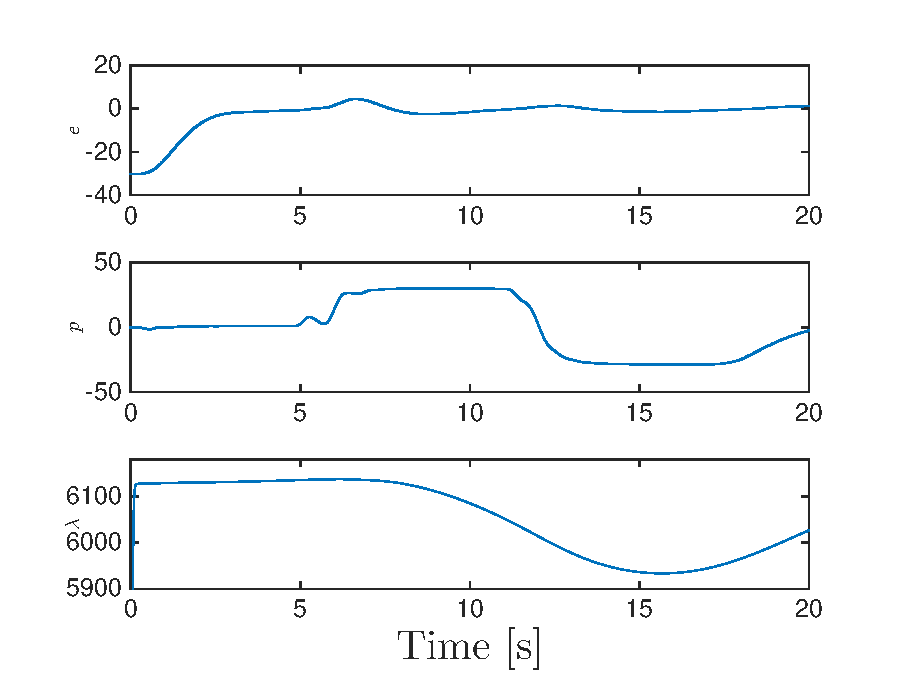
\includegraphics[width=\textwidth]{day2}
	\caption{Actual values day 2}
	\label{fig:day2}
\end{figure}

If we compare Figure \ref{fig:day2} and Figure \ref{fig:estimatedDay202}, we see that the travel values have a similar profile for the first 15 seconds or so, after which it starts to overcompensate (as described earlier). There is some deviation of pitch, with the actual pitch first swaying one way, and then back the other. We can also see that the elevation is not constant, as opposed to our earlier assumption.
\epigraph{\textit{'I've got 99 problems, but a pitch ain't one.'}}{Ice-T (1993)}

\section{Optimal control of pitch/travel with LQ control (10.3)}

%%%%%%%%%%%%%%%%%%%%%%%%%%%%%%%%%%%%%%%%%%%%%%%%%%%%%%%%%%%%
\subsection{LQ controller (10.3.1)}
%%%%%%%%%%%%%%%%%%%%%%%%%%%%%%%%%%%%%%%%%%%%%%%%%%%%%%%%%%%%

We introduce feedback to our system using the following manipulated variable:

\begin{equation}
	\V{u}_k = \V{u}_k^* - \M{K} \transpose (\V{x}_k - \V{x}_k^*)
\end{equation}
where $u_k^*$ and $x_k^*$ are the optimal input sequence and optimal trajectory calculated in the previous task. $\M{K}$ is the gain matrix, and can be calculated in numerous ways. We are going to determine it with an LQ (linear quadratic) controller that minimises the function

\begin{equation} \label{eq:LQcost}
	J = \sum\limits_{i=0}^{\infty} \Delta \V{x}_{i+1} \transpose \M{Q} \Delta \V{x}_{i+1} + \Delta \V{u}_{i} \transpose \M{R} \Delta \V{u}_{i}, \quad \M{Q} \geq 0, \, \M{R} > 0
\end{equation}
for the linear model

\begin{equation}
	 \Delta \V{x}_{i+1} = \M{A} \Delta \V{x}_{i} + \M{B} \Delta \V{u}_{i}
\end{equation}
where $\Delta \V{x} = \V{x} - \V{x}^*$ and $\Delta \V{u} = \V{u} - \V{u}^*$ are the deviations from the optimal trajectory. \eqref{eq:LQcost} can be solved in MATLAB using the function \texttt{dlqr}. 

\begin{figure}[H]
	\centering
	\includegraphics[width=\textwidth, trim=2cm 5cm 2cm 2cm]{simulinkmodels/heldag3}
	\caption{Simulink model of the system}
	\label{fig:heldag3}
\end{figure}

The behaviour of the helicopter is tuned by altering $\M{Q}$ and $R$, and by trial and error we obtained values that yielded descent behaviour of the helicopter:

\begin{equation}
	\M{Q} = 
    \begin{bmatrix}
    	25 & 0 & 0 & 0 \\
        0 & 0.5 & 0 & 0 \\
        0 & 0 & 100 & 0 \\
        0 & 0 & 0 & 0.5
    \end{bmatrix}
\end{equation}

\begin{equation}
	R = 1
\end{equation}

%%%%%%%%%%%%%%%%%%%%%%%%%%%%%%%%%%%%%%%%%%%%%%%%%%%%%%%%%%%%
\subsection{Behaviour with feedback (10.3.2)}
%%%%%%%%%%%%%%%%%%%%%%%%%%%%%%%%%%%%%%%%%%%%%%%%%%%%%%%%%%%%

The first thing we notice is that the helicopter now does come to a halt at the setpoint. In the plots of the measured states, you can see that the travel value is stationary from 19 seconds onwards. You can also see that travel overshoots very slightly, but stabilises nicely at $\lambda_f$.

\begin{figure}[H]
	\centering
	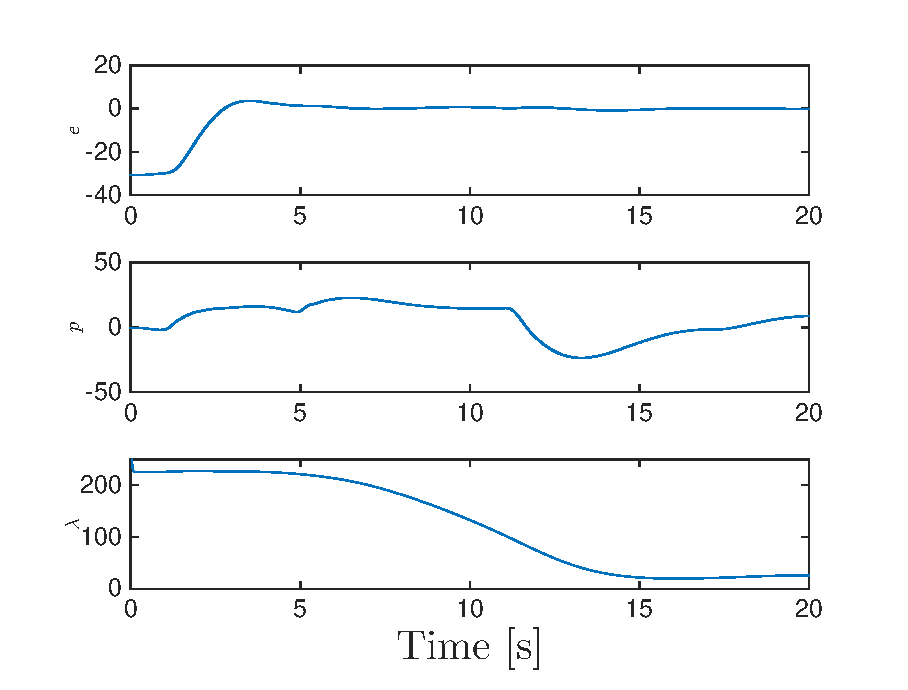
\includegraphics[width=\textwidth]{day3}
	\caption{Running the helicopter with feedback}
	\label{fig:day3}
\end{figure}


As shown the shape of both the travel and pitch match the calculated values found in \ref{fig:estimatedDay202} well. The feedback distorts the pitch from the calculated optimal as it works in parallel with the optimal input for the helikopter.

%%%%%%%%%%%%%%%%%%%%%%%%%%%%%%%%%%%%%%%%%%%%%%%%%%%%%%%%%%%%
\subsection{MPC discussion (10.3.3)}
%%%%%%%%%%%%%%%%%%%%%%%%%%%%%%%%%%%%%%%%%%%%%%%%%%%%%%%%%%%%

%%%%%%%%%%%%%%%%%%%%%%%%%%%%%%%%%%%%%%%%%%%%%%%%%%%%%%%%%%%%
\subsubsection{Realization of MPC}
%%%%%%%%%%%%%%%%%%%%%%%%%%%%%%%%%%%%%%%%%%%%%%%%%%%%%%%%%%%%
MPC can be realized with the following algorithm for linear MPC with state feedback

\begin{algorithmic}
\For{t = 0,1,2,...}
\State Get the current state $x_t$
\State Solve the convex QP problem on the prediction horizon from $t$ to $t+N$ with $x_t$ as the initial condition
\State Apply the first control move $u_t$ from the solution above
\EndFor
\end{algorithmic}

%%%%%%%%%%%%%%%%%%%%%%%%%%%%%%%%%%%%%%%%%%%%%%%%%%%%%%%%%%%%
\subsubsection{Advantages and disadvantages of using MPC)}
%%%%%%%%%%%%%%%%%%%%%%%%%%%%%%%%%%%%%%%%%%%%%%%%%%%%%%%%%%%%
There are both advantages and disadvantages with using an MPC controller compared to LQR.   
MPC requires a lot of computation, and may therefore require more expensive hardware or longer computation time. However, this can yield a very accurate controller. LQR is less computationally intensive, but also less accurate.

%%%%%%%%%%%%%%%%%%%%%%%%%%%%%%%%%%%%%%%%%%%%%%%%%%%%%%%%%%%%
\subsubsection{Figure 8 with MPC}
%%%%%%%%%%%%%%%%%%%%%%%%%%%%%%%%%%%%%%%%%%%%%%%%%%%%%%%%%%%%
\begin{figure}[H]
	\centering
	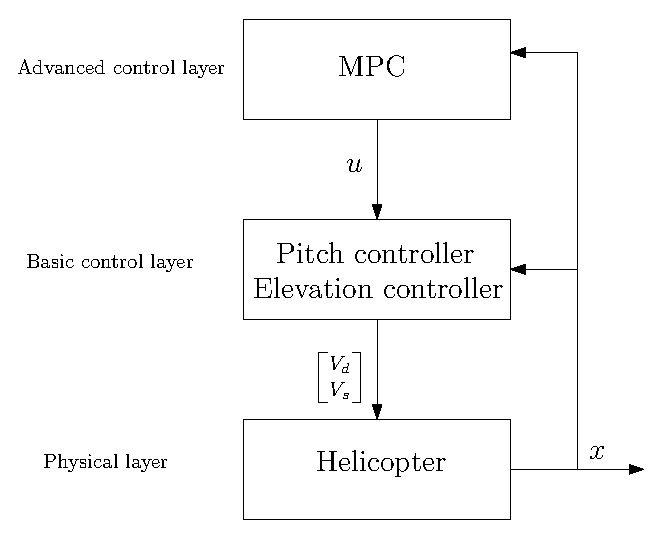
\includegraphics[width=10cm]{figurate_with_MPC}
	\caption{Figure 8 with MPC}
	\label{fig:figurate}
\end{figure}

The MPC, the pitch controller, and the elevation controller receives the measured position $x$ from the helicopter and calculates the input $u$, which the pitch and elevation controllers then use to find the voltages $V_d$ and $V_s$ to control the motors

\epigraph{\textit{'A helicopter does not want to fly, it just vibrates so much that the ground rejects it.'}}{Kurt Vonnegut}

\section{Optimal control of pitch/travel and elevation with and without feedback (10.4)}

%%%%%%%%%%%%%%%%%%%%%%%%%%%%%%%%%%%%%%%%%%%%%%%%%%%%%%%%%%%%
\subsection{Discretisation with elevation states (10.4.1)} \label{10.4.1}
%%%%%%%%%%%%%%%%%%%%%%%%%%%%%%%%%%%%%%%%%%%%%%%%%%%%%%%%%%%%
We will re-formulate the continuous system \eqref{eq:system} with additional states for elevation $e$ and elevation rate $\dot{e}$. The system with new state and input vectors \eqref{eq:state_input} and state equations \eqref{eq:state_eqns} is expressed by the matrices shown in \eqref{eq:matrices}.

\begin{equation}\label{eq:system}
	\V{\dot{x}}	= \M{A} \V{x} + \M{B} \V{u}
\end{equation}

\begin{equation}\label{eq:state_input}
	\V{x} =
	\begin{bmatrix}
		\lambda & r & p & \dot{p} & e & \dot{e}
	\end{bmatrix}\transpose
	,\qquad
	\V{u} =
	\begin{bmatrix}
		p_{c} & e_{c}
	\end{bmatrix}\transpose
\end{equation}

\begin{equation}\label{eq:state_eqns}
\begin{aligned}
	\dot{\lambda}	&= r \\
	\dot{r} 		&= - K_{2} p \\
	\dot{p}			&= \dot{p} \\
	\ddot{p}		&= K_{1} K_{pp} (p_{c} - p) - K_{1} K_{pd} \dot{p} \\
	\dot{e}			&= \dot{e} \\
	\ddot{e}		&= K_{3} K_{ep} (e_{c} - e) - K_{3} K_{ed} \dot{e}
\end{aligned}
\end{equation}

\begin{equation}\label{eq:matrices}
	\V{\dot{x}} =
	\underbrace{
		\begin{bmatrix}
			0 & 1 & 0				& 0				& 0				& 0				\\
			0 & 0 & -K_{2}			& 0				& 0				& 0				\\
			0 & 0 & 0				& 1				& 0				& 0				\\
			0 & 0 & -K_{1}K_{pp}	& -K_{1}K_{pd}	& 0				& 0				\\
			0 & 0 & 0				& 0 			& 0				& 1				\\
			0 & 0 & 0				& 0				& -K_{3}K_{ep}	& -K_{3}K_{ed}	\\
		\end{bmatrix}
	}_{\M{A}_{c}}
	\V{x} +
	\underbrace{
		\begin{bmatrix}
			0			& 0				\\
			0			& 0				\\
			0			& 0				\\
			K_{1}K_{pp}	& 0				\\
			0			& 0				\\
			0			& K_{3}K_{ep}	\\
		\end{bmatrix}
	}_{\M{B}_{c}}
	\V{u}
\end{equation}

%%%%%%%%%%%%%%%%%%%%%%%%%%%%%%%%%%%%%%%%%%%%%%%%%%%%%%%%%%%%
\subsection{Discretisation again (10.4.2)}
%%%%%%%%%%%%%%%%%%%%%%%%%%%%%%%%%%%%%%%%%%%%%%%%%%%%%%%%%%%%
As in Section \ref{sec:disc1}, we again need to discretize the system. The procedure is the same; refer to the earlier Section for clarification. The result can be seen in \eqref{eq:matrix_4.2_A} and \eqref{eq:matrix_4.2_B}.

\begin{equation}
\begin{aligned}
	\V{x}_{k+1}	&= \V{x}_{k} + \left( \M{A}_{c} \V{x}_{k} + \M{B}_{c} \V{u}_{k} \right) h \\
				&= \underbrace{\left( \Mc{I} + h \M{A}_{c} \right)}_{\M{A}} \V{x}_{k}
				+ \underbrace{h \M{B}_{c}}_{\M{B}} \V{u}_{k} \\
\end{aligned}
\end{equation}

\begin{equation}\label{eq:matrix_4.2_A}
	\M{A} =
	\begin{bmatrix}
		1 & h & 0				& 0					& 0				& 0					\\
		0 & 1 & -hK_{2}			& 0					& 0				& 0					\\
		0 & 0 & 1				& h					& 0				& 0					\\
		0 & 0 & -hK_{1}K_{pp}	& 1-hK_{1}K_{pd}	& 0				& 0					\\
		0 & 0 & 0				& 0					& 1				& h					\\
		0 & 0 & 0				& 0					& -hK_{3}K_{ep}	& 1-hK_{3}K_{ed}	\\
	\end{bmatrix}
\end{equation}

\begin{equation}\label{eq:matrix_4.2_B}
	\M{B} =
	\begin{bmatrix}
		0				& 0				\\
		0				& 0				\\
		0				& 0				\\
		hK_{1}K_{pp}	& 0				\\
		0				& 0				\\
		0				& hK_{3}K_{ep}	\\
	\end{bmatrix}
\end{equation}

%%%%%%%%%%%%%%%%%%%%%%%%%%%%%%%%%%%%%%%%%%%%%%%%%%%%%%%%%%%%
\subsection{Solution of the optimization problem (10.4.3)}
%%%%%%%%%%%%%%%%%%%%%%%%%%%%%%%%%%%%%%%%%%%%%%%%%%%%%%%%%%%%

The cost function is now extended to include the elevation state, which gives us \eqref{eq:cost_function_w_elev}, with constrains given by \eqref{eq:cost_constraint_w_elev}. 

\begin{equation} \label {eq:cost_function_w_elev}
	\phi = \sum\limits_{i=1}^N (\lambda_i - \lambda_f)^2 + q_1 p_{ci}^2 + q2 e_{ci}^2
\end{equation}

\begin{equation} \label{eq:cost_constraint_w_elev}
	\alpha \exp (-\beta (\lambda_k - \lambda_t)^2) -e_k \leq 0, \quad k \in \{ 1, ..., N \}
\end{equation}

In \eqref{eq:cost_constraint_w_elev}, we used the values $\alpha = 0.2$, $\beta = 20$ and $\lambda_t = \frac{2 \pi}{3}$.
We use \texttt{fmincon} to get the result of the cost function with the constraints. The parameters used are  \texttt{vlb} and \texttt{vub}, which are vectors containing the linear constraints; \texttt{mycon}, which returns the nonlinear constraints; and \texttt{Aeq} and \texttt{beq} which are the matrices for the problem to be solved. We also send in the cost function itself and the initial values \texttt{z0}.
\begin{lstlisting}
costf = @(z) 0.5*z'*Q*z;
z = fmincon(costf, z0, [], [], Aeq, beq, vlb, vub, @mycon);
\end{lstlisting}

%%%%%%%%%%%%%%%%%%%%%%%%%%%%%%%%%%%%%%%%%%%%%%%%%%%%%%%%%%%%
\subsection{Comparison of performance with and without feedback(10.4.4)}
%%%%%%%%%%%%%%%%%%%%%%%%%%%%%%%%%%%%%%%%%%%%%%%%%%%%%%%%%%%%
Without feedback the pitch goes to 0 when $\lambda = \lambda_f$, but does not compensate to avoid overshoot. With feedback, the helicopter will change its pitch to the opposite direction, making the helicopter stop and stay still at $\lambda = \lambda_f$. 

\begin{figure}[H]
	\centering
	\includegraphics[width=\textwidth, trim=2cm 5cm 2cm 2cm]{simulinkmodels/heldag4UnFeed}
	\caption{Simulink model of the system without feedback}
	\label{fig:heldag4UnFeed}
\end{figure}

\begin{figure}[H]
	\centering
	\includegraphics[width=\textwidth, trim=2cm 5cm 2cm 2cm]{simulinkmodels/heldag4medFeed}
	\caption{Simulink model of the system with feedback}
	\label{fig:heldag4medFeed}
\end{figure}

\begin{figure}[H]
	\centering
	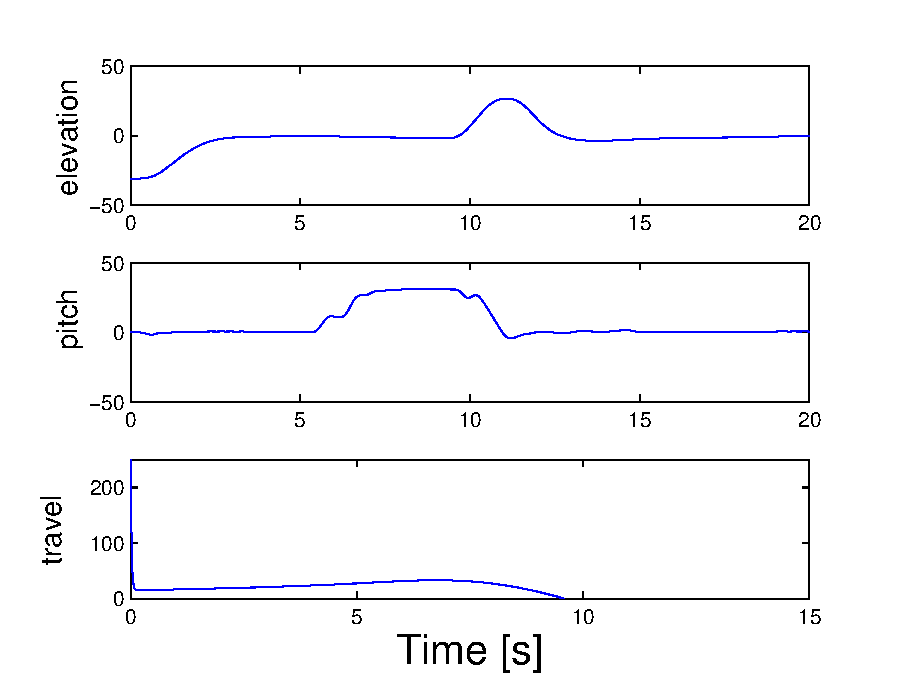
\includegraphics[width=\textwidth]{day4_nofeed}
	\caption{Actual values day 4 without feedback}
	\label{fig:day4nofeed}
\end{figure}


\begin{figure}[H]
	\centering
	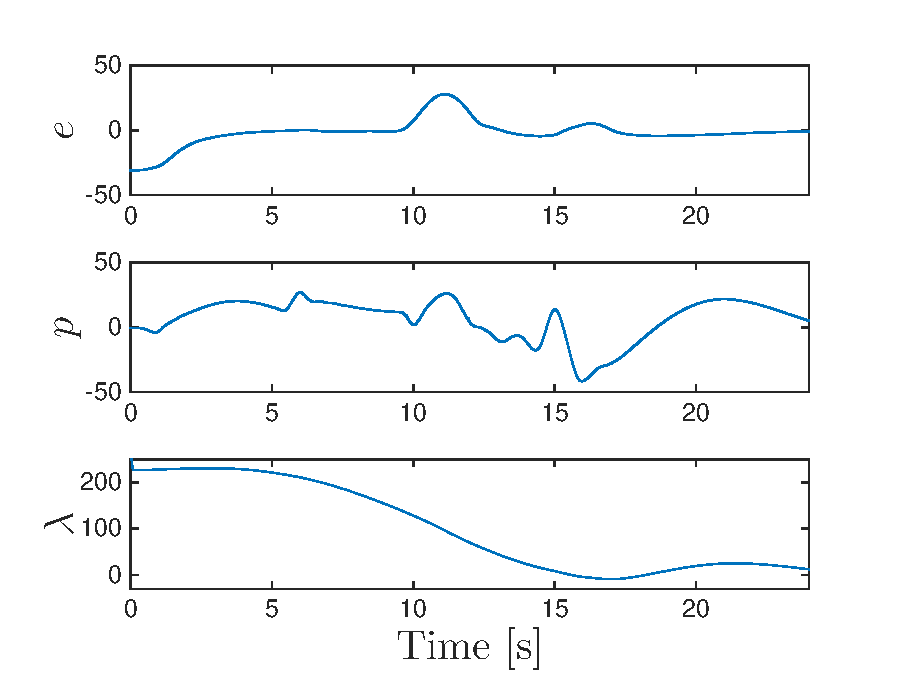
\includegraphics[width=\textwidth]{day4_yesfeed}
	\caption{Actual values day 4 with feedback}
	\label{fig:day4yesfeed}
\end{figure}

As we can see in the sensor data from the model without feedback, the helicopter does not stop at $\lambda = \lambda_f$, but keeps moving. In the model with feedback, however, it does stop at $\lambda = \lambda_f$, but the change in pitch to keep it still in the reference point also makes the helicopter elevate a bit, as can be seen in the plot at roughly 16 seconds. It also overshoots slightly, but converges at the setpoint.

In the calculated outputs you can see that it also expects some change in the pitch when trying to stop at the reference point, but it is much more subtle than the real behaviour, especially with feedback. This would correspond better if the LQR was tuned better. In the measured values of the model without feedback, this is more similar to the calculated pitch, but the travel is a bit off, as the helicopter keeps gliding after it reaches the reference point. This is improved in the model with feedback, although it does not stop as quickly and smoothly as the calculated output would suggest.

%%%%%%%%%%%%%%%%%%%%%%%%%%%%%%%%%%%%%%%%%%%%%%%%%%%%%%%%%%%%
\subsection{Discussion of decoupled states (10.4.5)}
%%%%%%%%%%%%%%%%%%%%%%%%%%%%%%%%%%%%%%%%%%%%%%%%%%%%%%%%%%%%
In real life the pitch and pitch rate of the helicopter would have an effect on both the elevation rate and the elevation itself. This will result in an offset from the calculated optimal trajectory.  
By modelling the system with the elevation and travel coupled with the pitch, you will remove the offset at the cost of a more complex model.
\section{Discussion}
The purpose of this lab was to formulate a dynamic optimization problem, and solve this using \texttt{MATLAB} and Simulink, as well as seeing the results of control both with and without feedback.

First, this was done by using model-based optimization to provide the pitch and elevation controllers with an input $u$, before the model was improved by adding an LQR-control layer between the optimization layer and the basic control layer. 


\section{Conclusion}

In conclusion our group feels that it has been interesting to work on this lab, and that we have learnt a lot by doing it. By getting a practical approach to implementing optimization algorithms, we have gained insight into how it can be to work as control system engineers and some of the problems they have to solve. 
We have also seen that using optimization algorithms when making a control system makes the system more precise, and is both worth the time and energy it takes to implement them. 

All in all we think this has been a successful exercise, that has been both rewarding and educational.
\section{Appendix}
\subsection{Variables}
\begin{center}
\begin{tabular}{l l l l}
\hline 
Symbol & Variable \\ \hline
$p$ & Pitch \\
$p_c$ & Setpoint for pitch \\
$\lambda$ & Travel \\
$r$ & Speed of travel \\
$r_c$ & Setpoint for speed of travel \\
$e$ & Elevation \\
$e_c$ & Setpoint for elevation \\
$V_f$ & voltage, motor in front \\
$V_b$ & Voltage, motor in back \\
$V_d$ & Voltage difference, $V_f -V_b$ \\
$V_s$ & Voltage sum, $V_f + V_b$ \\
$K_{pp}$, $K_{pd}$, $K_{ep}$, $K_{ei}$, $K_{ed}$ & Controller gains \\
$T_g$ & Moment needed to keep the helicopter flying
\end{tabular}
\end{center}
\label{table:variables}



\vspace{1cm}

\subsection{Constants}
\begin{center}
\begin{tabular}{l l l l}
\hline
Symbol & Parameter & Value & Unit \\ \hline
$l_a$ & Distance from elevation axis to helicopter body & 0.64 & m \\
$l_h$ & Distance from pitch axis to motor & 0.177 & m \\
$K_f$ & Distance from elevation axis to helicopter body & 0.1983 &\si{\newton \per \meter}  \\
$J_e$ & Moment of inertia for elevation & 1.0625 & \si{\kilogram \meter \squared}  \\
$J_t$ & Moment of inertia for travel & 1.0625 & \si{\kilogram \meter \squared}  \\
$J_p$ & Moment of inertia for pitch & 0.0406 & \si{\kilogram \meter \squared}  \\
$m_h$ & Mass of helicopter & 1.297 &\si{\kilogram}  \\
$m_w$ & Balance weight & 1.802 & \si{\kilogram} \\
$m_g$ & Effective mass of the helicopter & 0.026 & \si{\kilogram} \\
$K_p$ & Force to lift the helicopter from the ground & 0.2551 & \si{\newton}
\end{tabular}
\end{center}
\label{table:constants}



%\section{Pastebin (remove before handing in lol)}

%%%%%%%%%%%%%%%%%%%%%%%%%%%%%%%%%%%%%%%%%%%%%%%%%%%%%%%%%%%%
\subsection{Bibtex test}
%%%%%%%%%%%%%%%%%%%%%%%%%%%%%%%%%%%%%%%%%%%%%%%%%%%%%%%%%%%%
\cite{nocedal_numerical_2006} and \cite{_helicopter_2015} are pretty cool.

%%%%%%%%%%%%%%%%%%%%%%%%%%%%%%%%%%%%%%%%%%%%%%%%%%%%%%%%%%%%
\subsection{mcode test}
%%%%%%%%%%%%%%%%%%%%%%%%%%%%%%%%%%%%%%%%%%%%%%%%%%%%%%%%%%%%
\lstinputlisting[label={lst:dog}, caption={A dog.}]{blkdiag.m}

\begin{figure}[H]
	\centering
	\includegraphics[width=\textwidth]{Opp10_3-good}
	\caption{Digraph.}
	\label{fig:digraph}
\end{figure}


\bibliography{ref-helikopter}

\end{document}
